cl% Create simple notes latex docus
\section{Pipeline}
For the pipeline using docker and making docker the essential part of the pipeline.
Because of the necessity of docker in the pipeline, is because the scalability of the pipeline.
Docker also make the pipeline more portable, because of the docker images, that can be used on any machine.
If I dont have the possible of deploying the pipeline directly on another machines, the use
for the project fades away.

\section{Docker}
\label{sec:docker}
Docker plays a pivotal role in this project, serving as an integral tool. 
It offers a clean and efficient means of running instances that essentially 
need to be isolated once they have completed their execution. 
This allows for the encapsulation of the machines or infrastructure used for the \ac{CTF} within Docker images, 
which can then be shared with other systems. When these images are executed on those systems, the expectation is to achieve consistent outcomes.

Before delving into the Docker specifics, it's essential to understand Docker's networking capabilities.
Docker networking simplifies various aspects of network management.
It provides a mechanism for exposing Docker containers to the external world, enabling communication between containers,
and also enforcing isolation between them. This isolation is particularly vital. For instance,
if there's a Docker container running a webserver that needs to be accessible from the outside,
Docker's networking features come into play. You can create a dedicated Docker network and connect
the webserver container to it. 
Subsequently, other Docker containers can also be linked to this network, 
allowing them to communicate internally while remaining isolated from the external world, preventing unwanted access to the webserver.
\begin{figure}
    \centering
    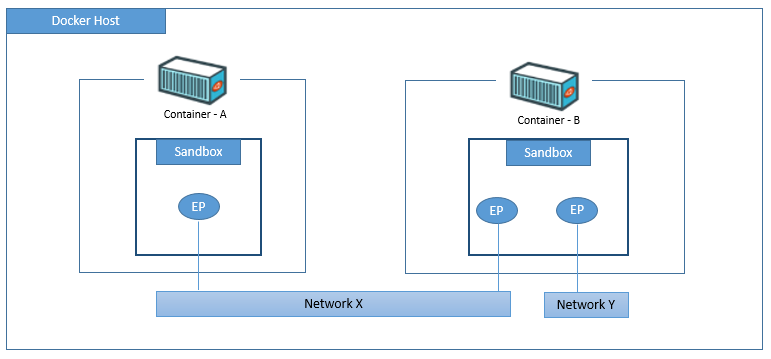
\includegraphics[width=0.8\textwidth]{images/docker_networks.png}
    \caption{Docker network}
    \label{fig:docker_network}
\end{figure}
Now as seen on the beautiful figure \ref{fig:docker_network} we have a docker network, which is called "network X".
Now as explained before every container attached to "network X" will be able to communicate with each other.
It can also talk to the outside world, but the outside can only talk to it, if I choose in my docker configuration to expose the container,
the port can be arbitrary.

Docker has a couple of different network types.
\begin{itemize}
    \item Bridge
    \item Host
    \item Overlay
    \item Macvlan
    \item None
\end{itemize}

Now I dont want to go into unnecessary details about the different network types, but I will explain the ones I have used in the project.
\subsection{Bridge}
In this project, I initially intended to utilize MacVlan,
but due to the fact that I'm running Docker on a uCloud platform where
the underlying hardware configuration seems to use IPVlan in conjunction with an external host server,
I had to resort to using a bridge. Consequently, each machine, essentially a Docker container,
behaves like a regular computer on a network. This has posed challenges because I
lack control over network-related aspects and cannot implement advanced functionalities.
The uCloud, or more specifically, the AAU-cluster network, is isolated from me. 
To perform any internal network tasks, I would need internet access, but the network restricts access
to anything other than SSH connections,
limiting my ability to carry out more advanced tasks.


\section{Drone CI/CD}

Drone\cite{droneio} is a CI/CD tool that is used to automate the process of building, testing and deploying software.
Drone is a container-native CI/CD platform built on Docker, written in Go. It uses a simple YAML configuration file,
and it leverages Docker, so it's easy to add support for new languages and frameworks.

Drone is a self-service solution that allows developers to build, test and deploy their own code.
It is designed to be easy to use, and it is built on top of Docker, so it is easy to add support for new languages and frameworks.

Also what very important about drone is that it is open source. Everything about the DroneAPI is open source and 
avaiable on their website. Now this tool seemed like the perfect tool for the job, because of the simplicity of the tool.
Running it together with gitea also seemed like a good idea, because of the integration between the two tools.
Boy was I wrong. 

\subsection{Drone problems}
\subsubsection{Problem 1, integration with gitea over OAuth2}
Other than starting out figuring out how to run drone, I had to figure out how to integrate it with gitea.
Now later version of drone, had its own database of users and therefore didn't have to rely on gitea for authentication.
Now this means that before being able to run drone runners to execute pipeline, the user that wish to use drone,
needs to authenticate with the gitea server, and post a access token to the gitea server. Essentially the user needs a token 
when is used to authenticate with the gitea server.
Now the authentication process is not a problem, the drone CI/CD documentation is very specific about how to do it and if done 
correctly it'll work fine.
Now the big problem is posting the token to the gitea server. The gitea server will not accept the token, being posted over http connection,
and it refusing the connection. 
Since drone need to make it's access token available to the gitea server, it needs to be able to post it to the gitea server.
The problem can be solved by using a proxy or a https connection on the gitea server, but that is not a viable solution.

\subsubsection{Problem 2, Advertised problem by drone}
Now the is linked to the first problem and is about the network aspect of drone.
The authentication of the user is done in the brower. WHen that is done drone obviously needs to be able to communicate with the gitea server.
Now the problem, and im not sure how docker compose works in this part, but what I've deciphered from the internet is that 
drone might not be able to find the gitea server, and post the token to it.

\subsubsection{Problem 3, Drone runner}
When the Drone server is operational, it acts as the intermediary connecting the Git server 
and the runners responsible for executing the pipeline. 
To ensure a smooth pipeline execution, it is imperative that the pipeline configuration 
for the Drone server is exceptionally detailed. This configuration should explicitly define 
crucial details such as the software used to manage the Drone server, particularly Docker if the Drone runners 
are tasked with running the pipeline within Docker containers.

Furthermore, the fact that this specification must be written in YAML introduces a 
level of dependency on YAML syntax and indentation. It's important to note that the 
specific syntax and indentation requirements can vary from one software platform to another when defining the structure of the pipeline. 
Therefore, careful attention to these details is vital to ensure accurate and effective pipeline execution.

\begin{figure}
    \begin{minted}[
        gobble=4,
        frame=single,
        linenos
      ]{yaml}
        kind: pipeline
        type: docker
        name: default
            
        steps:
        - name: backend
          image: golang
          commands:
          - go build
          - go test
            
        - name: frontend
          image: node
          commands:
          - npm install
          - npm run test
      \end{minted}
\end{figure}

\subsection{Problems with droneCI problematic}
Although the Drone CI/CD tool faced some challenges, I successfully configured it to run on the same machine as the Gitea server, 
even though the official Drone documentation doesn't recommend this approach. Furthermore, 
I managed to set up both the Drone server and Gitea within the same Docker network using Docker Compose. 
However, I encountered a significant issue that led me to reconsider Drone as a pipeline tool.

Following the authentication process using Gitea OAuth2, the Drone server requires the capability to post an access token to the Gitea database. 
This access token is crucial for the Drone server to authenticate interactions between itself and the Git server. 
Unfortunately, when the Drone server attempts to perform this operation, the Git server rejects the connection because it lacks an HTTPS connection. 
This conclusion is supported by the fact that when attempting to authenticate with `http://localhost:3000`, 
the Git server refuses the connection. However, when I connect the Drone server to a Git server running on an HTTPS connection, 
the Git server accepts the connection. The specific error is:
\begin{center}
  Post \url{"http://localhost:3000/login/oauth/access_token"}: dial tcp \url{127.0.0.1:3000}: connect: connection refused
\end{center}

Due to this limitation, the Drone server is not a viable option for our pipeline, as it 
necessitates the Git server to operate on an HTTPS connection. I would prefer the Git server 
to operate on an HTTP connection for the sake of pipeline simplicity.

I already proposed a solution and something that already has been done by is not a sustainable solution. 
Another solution which would was proposed on a blog page\cite{drone-solution-static-ip}. The solution is based of 
two things. One OAuth happens in the browers as mentioned either. Second, for the OAuth to happen, the drone 
server needs do the OAuth. But since it is exposed on localhost, it tries to authenticate with localhost ip, 
instead of the ip of the docker container. By specifying the ip of the docker container, the drone server will
be able to authenticate with the gitea server. This is not a sustainable solution, because the ip of the docker container
will change, if the docker container is restarted. This is not a viable solution, because the means that the image 
will become static and therefore might be subject to change.
